\documentclass[tikz, border=2pt]{standalone}

\usepackage{amsmath,amssymb}
\usepackage{pgfplots}
\pgfplotsset{compat=1.18}
\usepgfplotslibrary{groupplots}
\usetikzlibrary{arrows.meta}
\usepackage{xcolor}

\definecolor{utnblue}{RGB}{0, 51, 102}

\begin{document}
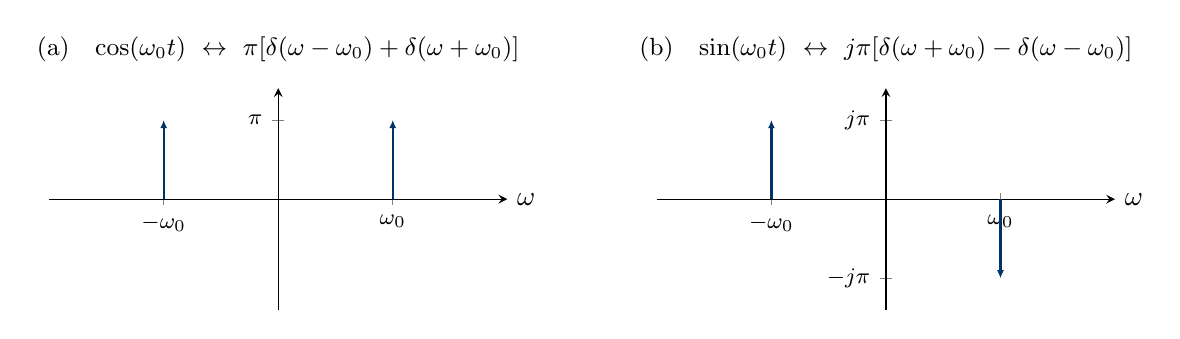
\begin{tikzpicture}[
    impulso/.style={utnblue, line width=0.8pt, -{Latex[length=3pt,width=2.6pt]}},
  ]

\begin{groupplot}[
    group style={group size=2 by 1, horizontal sep=1.9cm},
    width=7.4cm, height=4.4cm,
    axis lines=middle,
    enlargelimits=false,
    tick label style={font=\footnotesize},
    label style={font=\small},
    title style={font=\small},
    every axis x label/.style={at={(ticklabel* cs:1)}, anchor=west},
]

% --- Panel (a): TFTC de cos ---
\nextgroupplot[
    title={(a)\quad $\cos(\omega_0 t)\ \leftrightarrow\ \pi[\delta(\omega-\omega_0)+\delta(\omega+\omega_0)]$},
    xlabel={$\omega$},
    xmin=-4, xmax=4, ymin=-1.4, ymax=1.4,
    xtick={-2,2}, xticklabels={$-\omega_0$,$\omega_0$},
    ytick={1}, yticklabels={$\pi$},
]
\draw[impulso] (axis cs:-2,0) -- (axis cs:-2,1);
\draw[impulso] (axis cs: 2,0) -- (axis cs: 2,1);

% --- Panel (b): TFTC de sin (parte imaginaria) ---
\nextgroupplot[
    title={(b)\quad $\sin(\omega_0 t)\ \leftrightarrow\ j\pi[\delta(\omega+\omega_0)-\delta(\omega-\omega_0)]$},
    xlabel={$\omega$},
    xmin=-4, xmax=4, ymin=-1.4, ymax=1.4,
    xtick={-2,2}, xticklabels={$-\omega_0$,$\omega_0$},
    ytick={-1,1}, yticklabels={$-j\pi$,$j\pi$},
]
\draw[impulso] (axis cs:-2,0) -- (axis cs:-2,1);
\draw[impulso] (axis cs: 2,0) -- (axis cs: 2,-1);

\end{groupplot}

\end{tikzpicture}
\end{document}
